\section{Evaluation}
\label{sec:evaluation}

% Results figures, rendered from the persisted artifacts:
% bootstrap_ci.json (suite means and 95% CIs), stability_run1_vs_run2.json (run pairs).
% Layout discipline: the top panel shows point estimates + intervals only
% (no filled bars under the whiskers), the bottom panel's legend lives
% below the axis (never over the bars), and both panels share the same
% value range so the stacked scales read as one.
\begin{figure}[t]
\centering
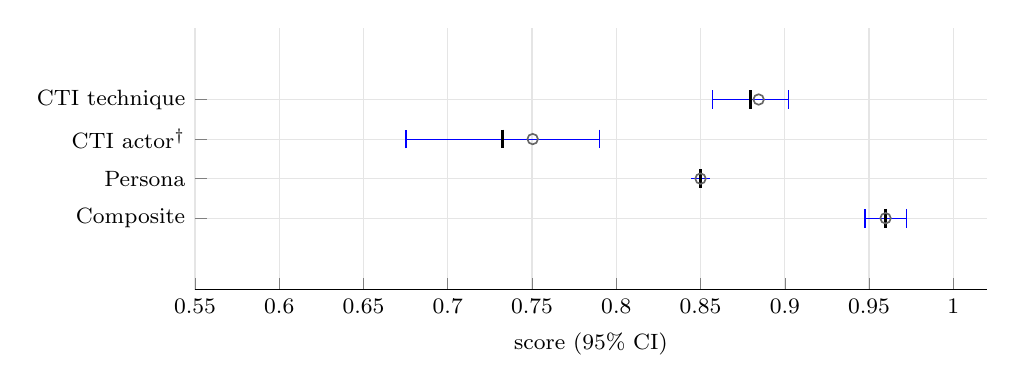
\begin{tikzpicture}
\begin{axis}[
  name=ax1,
  width=0.96\linewidth,
  height=4.9cm,
  xmin=0.55, xmax=1.02,
  y axis line style={draw=none},
  axis x line*=bottom,
  axis y line*=left,
  ytick=data,
  yticklabels={Composite,Persona,CTI actor$^{\dagger}$,CTI technique},
  y dir=reverse,
  xlabel={score (95\% CI)},
  xlabel style={font=\footnotesize},
  tick label style={font=\footnotesize},
  enlarge y limits=0.6,
  grid=major,
  grid style={black!10},
  clip=false
]
% point estimates and bootstrap 95% CIs from bootstrap_ci.json;
% only marks + intervals: no bars beneath the whiskers
\addplot+[only marks, mark=|, mark size=3.4, mark options={thick,black},
  error bars/.cd, x dir=both, x explicit] coordinates {
  (0.9598,3) +- (0.0122,0.0122)
  (0.8500,2) +- (0.0000,0.0000)
  (0.7325,1) +- (0.0573,0.0558)
  (0.8796,0) +- (0.0224,0.0204)
};
% run-2 overlay: open markers (point estimates from stability_run1_vs_run2.json;
% per-suite CIs were not computed for run 2, so none are drawn)
\addplot+[only marks, mark=o, mark size=1.9, mark options={semithick,black!60}] coordinates {
  (0.9598,3)
  (0.8500,2)
  (0.7504,1)
  (0.8845,0)
};
\end{axis}
\end{tikzpicture}

\vspace{2mm}

\begin{tikzpicture}
\begin{axis}[
  name=ax2,
  width=0.96\linewidth,
  height=4.9cm,
  ybar=1.5pt,
  bar width=9pt,
  ymin=0.55, ymax=1.0,
  symbolic x coords={CTI technique,CTI actor,Persona,Composite},
  xtick=data,
  ylabel={mean score},
  ylabel style={font=\footnotesize},
  tick label style={font=\footnotesize},
  ymajorgrids,
  grid style={black!10},
  enlarge x limits=0.25,
  legend style={font=\scriptsize, at={(0.5,-0.16)}, anchor=north, legend columns=2, draw=none, fill=none},
  legend cell align={left},
]
% run 1 vs run 2 from stability_run1_vs_run2.json
\addplot+[black!35, fill=black!35] coordinates {
  (CTI technique,0.9598) (CTI actor,0.8500) (Persona,0.7325) (Composite,0.8796)
};
\addplot+[black!70, fill=black!70, pattern=north east lines] coordinates {
  (CTI technique,0.9598) (CTI actor,0.8500) (Persona,0.7504) (Composite,0.8845)
};
\legend{run 1, run 2}
\end{axis}
\end{tikzpicture}
\caption{Live-campaign results from the persisted artifacts. \emph{Top:}
suite means with bootstrap 95\% confidence intervals; open markers mark
the independent second run's point estimates, and the actor interval is
degenerate ($^{\dagger}$) because the actor rubric assigns the same
score to every row, so uncertainty is carried by the Wilson pass-rate
interval instead (Table~\ref{tab:live}). \emph{Bottom:} two independent
218-query campaigns; the deterministic CTI strata replicate exactly and
only the LLM-judged persona stratum moves, by $+0.018$.}
\label{fig:results}
\end{figure}


The evaluation asks whether each mechanism the design introduces
contributes measurably, organized by the four research questions of
\S\ref{sec:intro}: the value of grounding (RQ1), consistency and safety
under adversarial interaction (RQ2), deception quality under an
independent LLM judge panel (RQ3), and the escalation pricing of each
intelligence rung (RQ4), followed by run-to-run stability and threats to
validity. Every quantitative claim in this section is traceable to a
persisted artifact in the released benchmark suite (Appendix~\ref{app:artifacts});
where an interval is reported it is a bootstrap 95\% confidence interval
computed over paired rows.

\subsection{Experimental Setup}
\label{sec:setup}

All experiments run on the production single-host deployment described in
\S\ref{sec:implementation} (2~vCPU, ${\sim}4$~GB RAM). Generative
components use two model families from one free-tier provider: a generator
for deception drafts and a judge model for evaluation, from a different
family than the generator; one catalog removal and one quota-exhaustion
window occurred during the study, both logged by the watcher and both
handled by the fallback path of \S\ref{sec:fallback}. Three query suites
exercise the loop end to end: \emph{CTI-technique} (123 queries on how
specific \attck techniques are abused), \emph{CTI-actor} (35 queries on
named threat-actor behavior), and \emph{persona-realism} (60 interactive
sessions driven by scripted attacker personas). One scope note: the
technique and actor suites are retrieval question-answering through the
loop's CTI path, not attacker interactions; the attacker-interaction
evidence is the persona stratum, the C1 re-query battery, and the
ablation/consensus scenarios. Each suite runs through the full verified
loop with HITL auditing enabled; the scenario sets are fixed and released,
so every run below is a re-run of the same 218 sessions.

Suite scores are normalized to $[0,1]$ with a per-scenario pass threshold;
composite is the row-weighted mean. The CTI suites are scored by fixed,
released string-matching rubrics, not by a model; their point structure,
and two consequences we state rather than let blur, are given in
Appendix~\ref{app:rubric-detail}: the rubrics measure the surface
delivery of the expected intelligence and cannot certify semantic
correctness (which is why the TTP-accuracy dimension of the consensus
study and the released transcripts matter); they are identical across
ablation arms, so the paired differential measures what grounding changes
about delivery, not extraction plumbing; and --- a defect not designed for
but caught by the manual audit of \S\ref{sec:scorer-audit} --- they credit
the expected identifier wherever it appears, including inside a fallback
template that echoes the attacker's query verbatim, so on template-dominated
runs the served-text channel overstates delivery. Served-text figures
below are raw-rubric values unless marked guarded. All intervals are
Wilson 95\% intervals for pass rates and percentile bootstrap 95\%
intervals (10{,}000 resamples, fixed seed) for continuous means; the code
and seed are released with the artifacts.

\subsection{RQ1: Does Grounding Change What the Honeypot Detects?}
\label{sec:rq1}

We run a 30-scenario-per-suite workload (the first 30 released scenarios
of each suite, fixed before the run) twice through the live loop: once
with retrieval grounding enabled and once with Don bypassed (prompts
otherwise identical), pairing every scenario across arms. The ablation
corpus is a subset of the campaign corpus, so the ablation and campaign
persona means are not comparable row-for-row (0.833 vs.\ 0.733; different
scenario subset and harness revisions between runs; the released per-row
rows make both decomposable).

\begin{table}[t]
\centering
\caption{Paired RAG-vs-no-RAG differential (90 pairs -- 30 per suite,
180 rows total; 95\% bootstrap CIs). Persona realism is predicted to be
retrieval-independent, and is.}
\label{tab:b4}
\begin{tabular}{lccc}
\toprule
Suite & RAG & No-RAG & $\Delta$ (95\% CI) \\
\midrule
CTI technique & 0.950 & 0.633 & $+0.317$ $[+0.162, +0.480]$ \\
CTI actor     & 0.850 & 0.710 & $+0.140$ $[+0.083, +0.197]$ \\
Persona       & 0.833 & 0.828 & $+0.005$ $[-0.047, +0.057]$ \\
\midrule
Overall (90 pairs) & & & $+0.154$ $[+0.092, +0.221]$ \\
\bottomrule
\end{tabular}
\end{table}

Table~\ref{tab:b4} (rendered per suite in
Appendix~\ref{app:figdetail}, the grounding render) shows the result:
grounding lifts technique detection by $+0.317$ and actor attribution by
$+0.140$, both intervals excluding zero, while the persona stratum is the
informative null -- its interval straddles zero, exactly as the
architecture predicts, because host-believability is produced by the
deception engine and the fiction graph, not by threat-intelligence
retrieval. An ablation that produced only wins would look manufactured;
this one discriminates. The mechanism claim is starker and is stated as a
dependence result, not a benefit: the grounded arm detects 35 distinct
TTPs across the campaign; the ungrounded arm detects none -- with
grounding disabled, every technique detection disappears (35 to 0),
which the architecture predicts, so the benefit claim rests on the
rubric-scored differential, not on the count. At the deployment level the
grounded arm passes 30 of 30 technique scenarios and the ungrounded arm
22 of 30, failing precisely the synthesis-shaped scenarios where static
templates have nothing to say. The deltas of Table~\ref{tab:b4} are
raw-rubric measurements, and the audit's echo guard bounds what they
certify: the ablation artifact does not persist served text, so the
guarded per-row differential cannot be recomputed; what the artifacts do
establish is arm-level asymmetry with text-independent instruments (35
distinct TTPs extracted from the grounded arm's transcripts, zero from
the ungrounded arm's) and the persona null, which needs no string rubric.
We state the delivery claim at that resolution rather than reusing a
number the audit has shown to be channel-contaminated
(\S\ref{sec:scorer-audit}).

\emph{Takeaway: grounding is responsible for the surface delivery of the
intelligence the system produces, the ablation localizes the effect to
exactly the suites that need it, and the raw detection count is a
dependence result the design entails, not an independent benefit.}

\emph{Verifier selectivity.} Across 2$\times$218 live-campaign rows the
verifier recorded zero rejections and the fallback path never engaged, so
the zero-unverified-serves result certifies the gate's coverage on that
workload, not its selectivity. Selectivity is measured where drafts are
actually induced to fail: an induced-failure red-team harness for the
verifier itself (labeled cases in eight categories) scores precision 1.000
and recall 1.000 across the now-96 canonical cases at the deterministic
stratum, and a live-LLM-authored stratum (236 drafts from one author
model, 261 from a second, over seven iterative rounds) reaches final
precision 1.000 (Wilson CI 0.977--1.000, zero false positives across 63
benign drafts) and recall 0.931/0.943 on the two authors, with every
fix pinned as a regression-locked canonical case. The full census, the
round-by-round verifier findings, and the residual missed-draft taxonomy
are given in Appendix~\ref{app:verifier-detail}; an over-rejecting
verifier degrades to the deterministic floor, never to silence, which is
why verifier false positives are themselves a safety property and are
reported as findings.

\subsection{RQ2: Consistency and Safety Under Adversarial Interaction}
\label{sec:rq2}

\emph{Fiction-graph consistency.} We re-query 45 facts across live
sessions (kernel versions, hostnames, listening services, database
engines, credentials) using adversarial phrasings designed to induce
drift, then compare each response against the session's fiction graph.
The graph-full configuration serves zero contradictions across 45
re-queries (95\% CI upper bound $0.079$), replays byte-identically,
records zero pinned-identity violations, and serves no response after a
failed verification verdict; the no-enforcement baseline provides none of
these properties (verifier coverage 45/45 turns versus 0). Two defects
this benchmark caught during development -- a credential template
recomputing timestamps from the wall clock mid-session, and a benign
\texttt{uname} re-query briefly flagged as a false contradiction -- are
documented with their fixes in Appendix~\ref{app:rq2-detail}; the verifier
now fails safe (unverifiable facts are rewritten or withheld, never served
on faith).

\emph{Predictive steering.} Across 10 predictions grounded in the session
corpora, top-3 next-technique accuracy is $0.9$, top-1 is $0.5$ (against
a kill-chain prior of ${\approx}0.4$ for single-label prediction), MRR is
$0.667$, and the steered bait reaches the plan in $0.9$ of sessions; the
A2 ablation confirms the bait signal comes from the steering context
(steer-to-plan $0.9 \to 0.4$).

\emph{Mechanism ablations.} The A1--A5 battery (Table~\ref{tab:ablations},
Appendix~\ref{app:rq2-detail}) removes one mechanism per configuration
and tests the goal from \S\ref{sec:goals} that motivated it: without the
fiction graph, plans lose fact binding; without bait steering,
steer-to-plan collapses; without the verifier, zero serves are verified;
without the HITL gate, require-class contents are served ungated; and the
linear fallback path is behaviorally equivalent when the graph adds no
information (A5, G4). All four mechanisms degrade as designed.

\subsubsection{Live campaign}
\begin{table}[t]
\centering
\caption{Live 218-query campaign (verified loop; Wilson pass-rate and
bootstrap mean CIs). Zero errors; 218/218 sessions engaged; 218/218
correct persona assignments; 132 TTPs (67 unique) detected with zero
false-positive CTI alerts, ground truth being the scenarios' expected
technique sets (no manual audit of campaign-scale extractions was
performed). Serve-path provenance: 88.1\% verified-generation serves,
11.9\% vetted deterministic, zero fallback serves (latency-split
estimate; see text).}
\label{tab:live}
\begin{tabular}{lccc}
\toprule
Suite & $n$ & Mean & 95\% CI \\
\midrule
CTI technique & 123 & 0.960 & $[0.948, 0.972]$ \\
CTI actor     & 35  & 0.850 & $[0.850, 0.850]^\dagger$ \\
Persona       & 60  & 0.733 & $[0.674, 0.788]$ \\
\midrule
Composite     & 218 & 0.880 & $[0.857, 0.900]$ \\
\bottomrule
\multicolumn{4}{l}{\footnotesize $^\dagger$Degenerate by construction: the actor rubric assigns the} \\
\multicolumn{4}{l}{\footnotesize same composite to every row, so the mean's bootstrap} \\
\multicolumn{4}{l}{\footnotesize interval carries no width; pass-rate uncertainty is} \\
\multicolumn{4}{l}{\footnotesize reported instead (Wilson $[0.901, 1.0]$).} \\
\end{tabular}
\end{table}
Table~\ref{tab:live} reports the full campaign and
Figure~\ref{fig:results} (top) renders the suite means with their
intervals. The persona stratum is the binding floor: 58 of 60 sessions
pass, and the failures are timeout-shaped turns under provider
safety-alignment pressure rather than deception failures (86.7\% of
generated turns on one commercial provider exceeded the inference
budget), consistent with the provider-fragility analysis of
\S\ref{sec:ethics}. The zero false-positive CTI alerts figure has known
ground truth: detections are counted against the campaign's scripted
scenarios, so the 132 detections and the zero false positives are the
same measurement read from both sides; the released per-row rows make the
claim checkable row by row. No manual audit of the 132 extractions was
performed; the consensus study's TTP-accuracy dimension samples exactly
this question, and a sampled manual audit of campaign-scale extractions
remains open.

\emph{Serve-path provenance.} Zero errors should not be read as the
deterministic path absorbing the campaign: a per-row analysis
(\path{serve_provenance.json}) attributes 88.1\% of run 1's serves (87.2\%
of run 2's) to the verified-generation path, the remainder to vetted
deterministic content. One honesty note: the split uses a 4\,s latency
threshold, not a per-row path flag (the harness recorded timing, not
provenance) -- stable at 2\,s, shifting at 10\,s to a bounded 88--77\% band;
the shift itself demonstrates the latency fingerprinting channel of
\S\ref{sec:threatmodel}. Decisively, \emph{fallback serves are zero}: the
fail-safe template swap never engaged -- the vetted share is the loop's
designed deterministic rung doing its job, not degradation.

\emph{Auditing the persona judge.} Because the persona stratum's
automated judge is a deterministic realism rubric, it can be audited
exhaustively offline against the transcripts it scored. Two systematic
errors surfaced: \emph{bait blindness} (correct canary bait deployments
scored $0.25$ against a rubric that penalizes brevity) and \emph{harness
contamination} (a session-echo bug row entering the deception mean at
$0.0$ despite measuring nothing about deception). The audit re-scores
both runs with three corrections; persona means move $0.733\to0.756$ and
$0.750\to0.762$, the canary-bias magnitude totals $2.1$ points on the
$[0,1]$ deception scale across the four audited runs, and both raw and
corrected means are released rather than silently substituted. The
correction was derived from and applied to the same corpus, so a
held-out validation with an independent judge model is named as required
future work; the audit chain is documented in
Appendix~\ref{sec:judgeaudit}.

\emph{Takeaway: the consistency and safety properties hold under targeted
adversarial pressure, and each mechanism in the loop is individually
necessary.}

\subsection{RQ3: Deception Quality Under an Independent LLM Judge
Panel}
\label{sec:rq3}

An LLM honeypot can be internally consistent and still be unconvincing,
so we score the end product -- with an evaluation panel, not a human
one. Eight ground-truth scenarios are executed live and the full
transcripts are scored on a 1--5 rubric (deception realism, persona
consistency, TTP accuracy, engagement, artifact safety) by three
evaluator personas: independently prompted LLM judges sharing one judge
model, chosen from a different family than the generator. Consensus is
the per-scenario mean across evaluators; exact agreement is $0.750$ -- a
within-model consistency figure, not inter-annotator agreement, and the
section heading is deliberately not ``human evaluators.'' The acceptance
bar was fixed in advance at a consensus of 3 per scenario. The consensus
score is $\mathbf{3.86/5}$, with all eight scenarios at or above the bar
(per-scenario rows in the released artifact, \path{results/human_eval_scored_20260922_180637_consensus/}); the weakest ($3.00$) is a web-application
SQLi hunt typed into a shell-scope honeypot -- the deception intent
holds, but the shell medium constrains persona realism, a scope boundary
we report rather than average away.


Three protocol details matter for interpreting the number. First,
evaluators score complete transcripts, not excerpts (an earlier truncated
scoring pass was rerun after we fixed the harness). Second, artifact
safety is scored against registered canaries: plaintext credential
material in a bait transcript is \emph{deployed deception}, not leakage.
Third, all three evaluators share one judge model; multi-model judging
was not possible on the provider at study time, and a panel of one
model's prompted personas is one evaluation instrument, however
partitioned -- the natural reading of \emph{independent judge panel} must
remain \emph{independent of the generator}, not independent across
judges. A small human-rater study over the eight released transcripts is
the obvious extension and is named as required future work. The panel's
remit is bounded by its medium: these judges read transcripts and never
experience the service's latency, so this study measures deception
content only.

\emph{Takeaway: the deception holds a three-evaluator consensus above the
acceptance bar on every scenario, with the failure modes named rather
than smoothed.}

\subsection{RQ4: Pricing the Ladder -- Adaptive Kind-Awareness and Its
Fold-Down}
\label{sec:jeveval}

The top rung of the ladder (\S\ref{sec:ladder}) is adaptive: a
kind-aware assessment layer that reads session behavior and returns the
attack kind and skill tier that the routing and deception layers should
act on. We price it in three experiments, each with its artifact
released; the full detail, census table, and funnel figure are in
Appendix~\ref{app:rq4-detail}.

\emph{Assessment quality on real logs.} On 13 replayed sessions drawn
from real Cowrie logs (captured live traffic against the isolated
testbed; expert-labeled severity ground truth, released with the
artifact), the baseline pipeline without kind-awareness correctly
assessed 0; with it, 12 of 13. The one miss was a session whose recorded
behavior was consistent with two kinds; we report the miss rather than
resolve it by hindsight. Thirteen sessions admit no meaningful
confidence interval, and the labels were assigned by the authors'
severity rubric, so this experiment is a directional case study, not a
powered comparison -- and it carries the section's most important
counter-signal, developed below.

\emph{Steering effect.} A 200-session stratified A/B on routing decisions
shows the ladder's descent in action. In the first pipeline revision,
kind-aware enrichment lifted routing accuracy from 69.5\% to 91.5\%,
fixing 44/44 misrouted APT sessions with zero regressions. The final
revision then reproduced that entire gain deterministically (an apt
skill-map repair, a weighted behavior-severity floor, and an n-gram
retrain of the classifier reaching 0.8875 $\to$ 0.9550 held-out
accuracy), leaving the assessment layer zero marginal accuracy
($\Delta = 0.0$, $n=200$). Because both arms sit at the pass ceiling,
we censused the full 400-session held-out corpus for the informative
stratum -- sessions whose deterministic routing lands below the tier
floor. It is small: six sessions, all APT-tier, from the classifier's
lower-confidence tail (mean confidence 0.53 versus 0.75 corpus-wide;
Table~\ref{tab:hardsunset}). Evaluated live on that stratum, one session
was rescued (transiently); the remaining five returned empty assessments
after provider refusals -- the free-tier endpoint refuses
security-shaped payloads, and a structured retry recovered none of the
five. The top rung's marginal effect on routing is therefore unmeasured
in both directions, and the removal stands on its measured record --
zero marginal effect on every row the benchmark resolves, zero
regression risk added by removal, a provider dependency eliminated --
with the bound stated rather than claimed away: \emph{no measurable
marginal effect at this benchmark's resolution}, not general subsumption.

\emph{Deception effect in closed loop.} Paired closed-loop replays pit a
simulated LLM attacker against the deception engine with and without
kind-aware guidance (97.8\% LLM-backed gateway calls, verified by a
canary echo probe after an earlier run was found to have silently
template-fallen back). Bait markers surfaced to the attacker rose from 4
to 9 (+125\%) across the five error-free family pairs -- a lexical count
over five pairs, no power, direction only. Dwell did not move: 34 vs.\
33 total turns in the clean paired comparison, the paired delta is
$-1$ turn, indistinguishable from noise -- a power-limited null, not an
established zero. The report's own mechanism analysis explains the null:
in both arms, nearly every early leave cites inconsistent fictional
filesystem state, so response consistency, not deception style, is the
binding constraint. This is precisely why the fiction graph and verifier
sit below the adaptive layer in the ladder.

\emph{Takeaway: the top rung buys assessment coverage and bait exposure,
not dwell time -- and its routing contribution, unresolvable at the
benchmark's ceiling and unavailable on the rows that matter most, was
compiled down to a deterministic floor. The counter-signal is stated
with equal weight: on the 13 real-log sessions, the deterministic floor
misjudged every severity (0/13 at expert level) while the assessed rung
corrected 12 -- the synthetic ceiling and the real-log collapse are the
domain-shift gap in both directions, and they are exactly why the
removal claim is bounded to this benchmark rather than generalized.}

\subsection{Scorer-Validity Audit: Manual Annotation of the CTI
Channels}
\label{sec:scorer-audit}

Every deterministic rubric above is itself a measurement instrument, so
we audited the two CTI channels against manual annotation: the full
218-query workload re-collected with served text persisted per row,
packaged into blinded packets, labeled by two independent annotators
(fixed-identity open-weights models standing in for the release plan's
human raters) with a third adjudicating, taxonomy pinned to \attck{}
Enterprise v19.1 (sha256-locked). The annotators agree with each other
at $\kappa = 0.866$ on technique identification; adjudicated labels
agree with the machine's \emph{analysis}-channel verdicts at
$\kappa = +0.75$ (TPR 0.992) -- the Don channel's 0.960 and 0.850
averages measure real extraction, not scorer artifacts.

The served-text channel did not survive its own audit. On technique
rows, 67 of the 71 machine-positive verdicts have one mechanical cause:
the served text is a fallback template echoing the attacker's query
verbatim, and the string rubric credits error text (the same mechanism
explains all 33 machine-positive actor verdicts). Echo-guarding the
scorers collapses the audited surface's served-text means from 0.524 to
0.057 (technique) and 0.680 to 0.000 (actor), and machine-vs-human
agreement rises from $\kappa = -0.19$ to $+0.35$ (technique) and from
$0.05$ to $0.91$ (actor): the guarded machine now agrees with the human
labels it previously contradicted. Because the audited surface was
proven row-identical to the current configurations' re-runs (pre-guard
score equality on all 218 rows), the guarded numbers are the corrected
values for the released two-channel artifact
(full guarded/raw columns in the released two-channel artifact). On the
campaign's persisted response previews, 61 of 123 technique rows and 25
of 35 actor rows are echo templates, with guarded served-text-only means
$\geq 0.107$ (technique) and $\geq 0.163$ (actor) against raw
both-channel figures of 0.960 and 0.850. Three properties are unchanged
by the correction and none depends on a string rubric: the
zero-unverified-serves result and the verifier's red-team precision and
recall; every paired per-row delta in the external-baseline ladder,
whose compared arms serve byte-identical strings; and the analysis
channel itself. What the correction removes is the claim that the CTI
suites' \emph{served} text carried the expected intelligence on this
infrastructure: the analysis channel carried the value, and the
two-channel declaration -- adopted before the audit -- is what kept the
two findings separable. The persona suite is untouched: its 60 rows
score identically raw and guarded (0.649), and its quality evidence is
the judge-panel consensus study, not a string rubric. Full annotation
detail and the blinded-audit tables ship in the released artifact.

\subsection{External Baselines}
\label{sec:external}

\begin{table}[t]
\centering
\caption{External baselines on the 218-query workload (generator:
deepseek-v4-flash-free for all LLM arms). \textbf{All scores are
served-text channel under the raw (pre-guard) rubric}---the deception
quality an attacker experiences. Paired per-row deltas are
scorer-invariant: the verified loop serves byte-identical strings to the
no-verifier arm on all 218 rows (paired delta 0.000), and the
host-fiction layer adds cross-session consistency at exactly zero
quality cost (paired per-row delta 0.000). Absolute levels on
fallback-heavy runs shift under the echo guard
(per the released two-channel artifact); the grounding and consistency contrasts
do not.}
\label{tab:baseline-served-text}
\begin{tabular}{lc}
\toprule
Arm & Served-text composite \\
\midrule
Vanilla Cowrie (no LLM) & 0.001 \\
Stateful LLM (HoneyGPT/LLM-SSHH) & 0.070 \\
Bare LLM (unverified) & 0.502 \\
RAGIN w/o verifier & 0.618 \\
RAGIN full (verified loop) & 0.618 \\
RAGIN full + host fiction & 0.618 \\
\bottomrule
\end{tabular}
\end{table}

Table~\ref{tab:baseline-served-text} places the loop against practice on
the version-of-record workload (vanilla Cowrie, a stateful LLM, an
unverified LLM, and RAG-without-verifier variants,
generator-held-fixed; \path{external_baseline_model_coherent.json}). Its
paired per-row deltas are the durable content, while its CTI-suite
absolute levels are fallback-dominated and are reported raw under the
declared served-text channel with the guard analysis of
\S\ref{sec:scorer-audit} applied where the persisted surface allows. What
remains open is the guarded regeneration of the CTI suites on a
healthy-generation window with full-transcript persistence --- the field
campaign's collection path now persists both.

\emph{Traditional-baseline head-to-head.} A separate comparison against
vanilla Cowrie (\path{cowrie_comparison.json}, regenerated from the
committed merged log \path{data/cowrie_logs/cowrie_merged.json}) gives:
Cowrie 16 sessions, engagement 0.812, 10 unique TTPs, composite 0.412;
RAGIN 30 sessions, 0.960, 13 unique, 0.697; $\Delta$ composite
$+0.284$. Two caveats govern its reading. First, both sides are
driver-generated: every Cowrie session in the committed logs originates
from the benchmark driver over the local Docker bridge, and no
external-attacker Cowrie session exists in any committed log, so this
is a harness-to-harness comparison, not a field measurement. Second,
the samples are small (16 vs.\ 30) and unequal in kind (single-turn
probe sessions versus the multi-turn loop), which is why we report it
as directional evidence that the harness runs against a traditional
baseline without modification -- Cowrie has no honeytoken engine and no
fiction machinery, so the composite dimensions it cannot attempt
depress its score by construction.

\subsection{Run-to-Run Stability}
\label{sec:stability}

LLM-driven systems rarely report whether their numbers replicate, so we
ran the full 218-query campaign twice, independently, with identical
configuration (Figure~\ref{fig:results}, bottom). The composite moves
from $0.880$ to $0.884$ ($\Delta +0.005$); per-row pass-decision
agreement is $0.991$ (216 of 218 rows). The deterministic strata
reproduce exactly (per-row mean absolute difference $0.000$); the
persona stratum, the only LLM-judged stratum, shows MAD $0.096$ with
pass agreement $0.967$. The headline metrics are identical across runs:
132 TTPs, 67 unique, 218/218 engagement, 218/218 persona assignment.
Recomputed on the judge-audited rows, the comparison is unchanged
($0.883\to0.888$, $\Delta+0.005$, same $0.991$ agreement), and both raw
and audited comparisons carry the same verdict (stable) in the persisted
artifact. Two caveats are recorded with the numbers: the run-to-run
variance is generator-side (32 of 60 persona rows differ between runs,
only one touched by the audit), and on the CTI suites the two runs'
per-row score equality is template-assignment determinism, not content
determinism -- under the echo guard the runs' guarded served-text means
separate (0.479 vs.\ 0.455 technique, computed on persisted previews) --
so the deterministic-strata reproduction claim, true of the recorded
scores, must not be read as transcript identity. The audited-stability
reconciliation detail is in Appendix~\ref{sec:judgeaudit}.

\subsection{Threats to Validity}
\label{sec:threats}

\emph{Construct.} Suite scores reward grounded technique coverage; a
system could game them by keyword stuffing. The persona rubric and the
judge-panel consensus study exist partly to catch exactly that failure,
and the two agree --- and the echo-credit failure the manual audit
caught (\S\ref{sec:scorer-audit}) is precisely this defect class,
realized not by an adversary but by the system's own fallback path; the
guarded scorers, the audit artifact, and the raw-vs-guarded columns of
The guarded/raw columns of the released artifact now bound it. \emph{Internal.} The judge
model shares a provider with the generator (different family); the
consensus protocol, rubric corrections, and the deterministic strata
bound but do not eliminate provider-common-mode effects, and the judge
panel is one model however partitioned, so the quality study has no
inter-judge or human component. The rubric corrections were derived and
applied on the same corpus. \emph{External.} The deployment observes
tailnet traffic only: no ambient internet background radiation, no
botnet churn, no real APT dwell time; the live fleet runs one SSH
listener plus HTTP and Telnet services, so web-shaped attack surfaces
are under-represented. The workload personas approximate but do not
replace live adversaries. The routing corpus is synthetic and the
floor's patterns were tuned against its generator, so the fold-down
ceiling is in-sample for the tuning process; the 13-session real-log
study points the other way and is too small to resolve. \emph{Statistical.}
Bootstrap CIs are computed over paired rows (percentile, 10{,}000
resamples, fixed seed); Wilson intervals are used for pass rates;
scenario counts per suite (35--123) bound interval width. The RQ4
comparisons are power-limited throughout (13 real-log sessions, five
replay pairs, six informative census rows, ten steering predictions) and
are priced as directional evidence, not established effects. The
external baselines of \S\ref{sec:external} are served-text-channel and
fallback-dominated in their CTI absolute levels, as declared above.